
\documentclass[a4paper,fleqn,usenatbib]{mnras}

\usepackage{newtxtext,newtxmath}
% Depending on your LaTeX fonts installation, you might get better results with one of these:
%\usepackage{mathptmx}
%\usepackage{txfonts}

\usepackage[T1]{fontenc}
\usepackage{ae,aecompl}


\usepackage{graphicx}	% Including figure files
\usepackage{amsmath}	% Advanced maths commands
\usepackage{amssymb}	% Extra maths symbols

%%%%%%%%%%%%%%%%%%%%%%%%%%%%%%%%%%%%%%%%%%%%%%%%%%

%%%%% AUTHORS - PLACE YOUR OWN COMMANDS HERE %%%%%

% Please keep new commands to a minimum, and use \newcommand not \def to avoid
% overwriting existing commands. Example:
%\newcommand{\pcm}{\,cm$^{-2}$}	% per cm-squared

%%%%%%%%%%%%%%%%%%%%%%%%%%%%%%%%%%%%%%%%%%%%%%%%%%


% Title of the paper, and the short title which is used in the headers.
% Keep the title short and informative.
\title[Research is fun, max. 45 characters]{You can't spell Euphoric without Eu.}

% The list of authors, and the short list which is used in the headers.
% If you need two or more lines of authors, add an extra line using \newauthor
\author[Matthew T. Miles et al.]{
Matthew T. Miles,$^{1}$\thanks{E-mail: mtmil3@student.monash.edu}
A. N. Other,$^{2}$
Third Author$^{2,3}$
and Fourth Author$^{3}$
\\
% List of institutions
$^{1}$School of Physics and Astronomy, Monash University, Clayton Campus, Victoria 3800\\
$^{2}$Department, Institution, Street Address, City Postal Code, Country\\
$^{3}$Another Department, Different Institution, Street Address, City Postal Code, Country
}

\date{Accepted XXX. Received YYY; in original form ZZZ}

\pubyear{2015}

\begin{document}
\label{firstpage}
\pagerange{\pageref{firstpage}--\pageref{lastpage}}
\maketitle

\begin{abstract}
This is a simple template for authors to write new MNRAS papers.
The abstract should briefly describe the aims, methods, and main results of the paper.
It should be a single paragraph not more than 250 words (200 words for Letters).
No references should appear in the abstract.
\end{abstract}

\begin{keywords}
keyword1 -- keyword2 -- keyword3
\end{keywords}


\section{Introduction}



Heavy elements (those with an atomic number greater than 30) must be synthesized using the slow (s) and rapid (r) neutron capture processes (\cite{Sneden2008}). The creation and abundance of these elements has been a key area in astrophysics research, and has been discussed and debated ever since the idea was first introduced in 1957 (\cite{Burbidge1957}). In the particular case of Europium (atomic number 63), almost all is produced through the r-process. The r-process occurs under very specific circumstances, where the neutron density is high enough that the rate of neutron capture will occur faster than the rate at which the element undergoes a $\beta$ decay. The sites at which this phenomena can occur are very specific, with the most favoured being early core-collapse supernovae which would have enriched gas clouds that later led to enriched star formation. Or more recently, neutron star mergers, as is theorised to have occurred in the case of the highly r-processed enhanced ultra-faint dwarf (UFD) galaxy Reticulum II (\cite{Ji2016}).

The recent discovery of the UFD Reticulum II has sparked discussion about the origin of r-process elements. Historically UFD's have had some of the lowest abundance of r-process elements of any celestial body, however analysis of several of Reticulum II's stars show they are greatly enriched, to the factor of 2-3 orders of magnitude higher than stars found in any other UFD (\cite{Ji2016}). This measure of enrichment lends evidence to the theory that a single rare event (such as a neutron star merger) must have occurred in the galaxies formative years to enrich it, as (for Europium especially) the heavy element yields are found to be 1000 times higher than would be achieved from core-collapse supernovae ejecta. 

While core-collapse supernovae and neutron star mergers are likely to be the progenitors of most r-process material, that is not to say that all r-process material stems from these sources. Rather it might serve as an indication of the rarity of stars found to be enhanced in these elements. 
\\\\
The second data release from the LAMOST telescope catalogued close to 2 million spectra (low resolution) of giant stars. Of these 2 million, 454,180 were fit against a normalised spectra from a sample of 9952 giants by Anna Ho (\cite{AnnaHo2017}), and from this it became possible to analyse which giants showed an abundance or depletion of particular heavy elements. 

In this letter we report the probable discovery of 22 of these LAMOST giants that show enhanced r-process peaks for Europium at both 4129 and 4205 Angstroms. The giants belong to a broad range of both metallicity and temperature, and don't cluster or trend towards any particular place in the observed sky. These characteristics and seeming lack-of a trend could argue that the mechanism that created these r-process enhanced stars may be general for all similar giant stars. 



\section{Methods, Observations, Simulations etc.}
Normally the next section describes the techniques the authors used.
It is frequently split into subsections, such as Section~\ref{sec:maths} below.

\subsection{Observations}
The 

\subsection{Maths}
\label{sec:maths} 

Simple mathematics can be inserted into the flow of the text e.g. $2\times3=6$
or $v=220$\,km\,s$^{-1}$, but more complicated expressions should be entered
as a numbered equation:

\begin{equation}
    x=\frac{-b\pm\sqrt{b^2-4ac}}{2a}.
	\label{eq:quadratic}
\end{equation}

Refer back to them as e.g. equation~(\ref{eq:quadratic}).

\subsection{Figures and tables}

Figures and tables should be placed at logical positions in the text. Don't
worry about the exact layout, which will be handled by the publishers.

Figures are referred to as e.g. Fig.~\ref{fig:example_figure}, and tables as
e.g. Table~\ref{tab:example_table}.

\begin{figure}
	% To include a figure from a file named example.*
	% Allowable file formats are eps or ps if compiling using latex
	% or pdf, png, jpg if compiling using pdflatex
	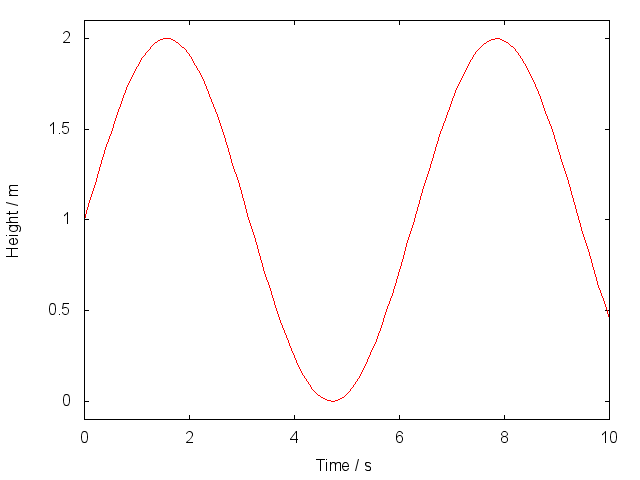
\includegraphics[width=\columnwidth]{example}
    \caption{This is an example figure. Captions appear below each figure.
	Give enough detail for the reader to understand what they're looking at,
	but leave detailed discussion to the main body of the text.}
    \label{fig:example_figure}
\end{figure}


\begin{table}
	\centering
	\caption{This is an example table. Captions appear above each table.
	Remember to define the quantities, symbols and units used.}
	\label{tab:example_table}
	\begin{tabular}{lccr} % four columns, alignment for each
		\hline
		A & B & C & D\\
		\hline
		1 & 2 & 3 & 4\\
		2 & 4 & 6 & 8\\
		3 & 5 & 7 & 9\\
		\hline
	\end{tabular}
\end{table}


\section{Conclusions}

The last numbered section should briefly summarise what has been done, and describe
the final conclusions which the authors draw from their work.

\section*{Acknowledgements}

The Acknowledgements section is not numbered. Here you can thank helpful
colleagues, acknowledge funding agencies, telescopes and facilities used etc.
Try to keep it short.


% The best way to enter references is to use BibTeX:

\bibliographystyle{mnras}
\bibliography{paper} % if your bibtex file is called example.bib
\begin{thebibliography}{99}
	\bibitem[\protect\citeauthoryear{Sneden, Christopher; Cowan, John J; Gallino, Roberto}{2008}]{Sneden2008}
	Sneden C., Cowan J.J., \& Gallino R. 2013, Annual review of Astronomy \& Astrophysics, 46, 1
	\bibitem[\protect\citeauthoryear{Ji, Alexander P.; Frebel, Anna; Chiti, Anirudh; Simon, Joshua D.}{2016}]{Ji2016}
	Ji A. P., Frebel A., Chiti A., \& Simon J. D. 2016, Nature, 531
	\bibitem[\protect\citeauthoryear{Ho, Anna Y.Q; Ness, Melissa K; Hogg, David W; Rix, Hans-Walter; Liu, Chao,; Yang, Fan; Zhang, Yong; Hou Yonhui; Wang Yuefei}{2017}]{AnnaHo2017}
	Ho A. Y. Q., Ness M. K., Hogg David W., Rix H-W., Liu C., Yang F., Zhang Y., Hou Y.,\& Wang Y. 2017, ApJ, 836, 1
	\bibitem[\protect\citeauthoryear{Burbidge, E. Margaret; Burbidge, G.R.; Fowler, William A.; Hoyle, F}{1957}]{Burbidge1957}
	Burbidge E. M., Burbidge G. R., Fowler W. A., \& Hoyle F. 1957, Review of Modern Physics, 29, 4
\end{thebibliography}



\appendix

\section{Some extra material}

If you want to present additional material which would interrupt the flow of the main paper,
it can be placed in an Appendix which appears after the list of references.

% Don't change these lines
%\bsp	% typesetting comment
\label{lastpage}
\end{document}
